\chapter{Literature Review} \label{chapter:lit_review}

Algorithmic recourse was first defined in the machine learning literature as ``the ability of a person to obtain a desired outcome from a fixed model'' \citep{ustunActionableRecourseLinear2019}. In our example from the introduction, where you are declined a mortgage, the digital bank provides recourse in the form of an alternative set of features (also referred to in the literature as `flipsets'). Should you change your features to the alternative set of features (where your income is £70,000 and savings are £40,000), then the mortgage will be approved (a positive outcome). In this example, the digital bank's mortgage approval classifier is fixed - the alternative set of features will not result in the mortgage being declined again when you re-apply.


\section{Problem Formulation}
The algorithmic recourse problem can be defined formally as shown in equation \ref{eq:recourse_setup}, where an individuals' original features are $\mathbf{x}$, $h: \mathbb{R}^D \to \{0,1\}$ is the classifier and $\mathcal{F}$ is the set of feasible features values. The set of feasible feature values constrains $\mathbf{x}'$ by only allowing positive/integer/similar constraints values of $\mathbf{x}'_i$ where relevant (e.g, number of credit cards must be either 0 or a positive integer, credit score must be between 0 and 999\footnote{Experian credit scores run from 0-999, see link \href{https://www.experian.co.uk/consumer/experian-credit-score.html}{here}.}). For \textit{immutable} variables (e.g., race, birthplace, etc.) it must be that the new feature value is the same as the original, that is $\mathbf{x}_i=\mathbf{x}'_i$.

\begin{align} \label{eq:recourse_setup}
	\mathbf{x}^* = & \argmin_{\mathbf{x}'}  \cost(\mathbf{x}, \mathbf{x}') \\ \nonumber
	\text{s.t. } & h(\mathbf{x}') = 1, \\ \nonumber
	& \mathbf{x}' \in \mathcal{F}
\end{align}

\section{Cost Functions} \label{section:cost_functions_lit_review}

Typically, the cost function is either of the form $L_p(\mathbf{x}'-\mathbf{x}')$, with the $L_1$ and $L_2$ norm being the most common \citep{ramakrishnanSynthesizingActionSequences2020, karimiSurveyAlgorithmicRecourse2022}. For the $L_1$ and $L_2$ norms, this cost function is always greater than or equal to 0, and is minimised when $\mathbf{x} =\mathbf{x}'$. The further away from the original features $\mathbf{x}$ that the counterfactual values $\mathbf{x}'$ are, the higher the cost. Intuitively, this means that leaving the features unchanged will result in a cost of 0, whilst significant changes (either positive or negative) will occur a cost that increases with the size of the changes.\\

Another function prevalent in the algorithmic recourse literature is the total log percentile shift \citep{ustunActionableRecourseLinear2019}, shown in equation \ref{eq:total_log_percentile_shift}, where $D$ is the number of features and $Q_i$ represents the CDF of $\mathbf{x}_i$. This cost function also considers the cost of each feature changed independently. It punishes increasing from the percentile $Q_i(\mathbf{x}'_i)$ is larger than the original percentile $Q_i(\mathbf{x}_i)$. A key advantage of this cost function is that changes become harder when starting from a higher percentile, e.g, moving from the 50$^{\text{th}}$ to 55$^{\text{th}}$ percentile carries a cost of 0.105, where as moving from the 90$^{\text{th}}$ to 95$^{\text{th}}$ percentile carries a cost of 0.693. This is likely to reflect reality more than the same cost for increasing percentile by 5 percentage points. Whilst the cost is 0 when $\mathbf{x}_i = \mathbf{x}'_i$, it becomes negative when $Q_i(\mathbf{x}'_i) < Q_i(\mathbf{x}_i)$. Therefore, for this cost function to applied correctly, it requires a monotonic constraint (e.g. increasing income is positively associated with credit score)\comment{improve this}.

\begin{equation} \label{eq:total_log_percentile_shift}
	\cost(\mathbf{x}, \mathbf{x}') = \sum_{i=1}^D \log \bigg( \frac{1 - Q_i(\mathbf{x}_i)}{1 - Q_i(\mathbf{x}_i')} \bigg)
\end{equation}

A related branch of literature, \textit{strategic classification}, studies the effect of the behaviour of strategic agents on classifiers. Individuals strategically manipulate their features in order to gain a favourable outcome, as opposed to increasing the underlying variable being classified, for example `credit-worthiness' in a credit scoring setting or practical skills relevant to a specific job in the hiring setting. Designing strategy-robust classifiers or classifiers that incentivise improvement requires a cost function of changing features from $\mathbf{x}$ to $\mathbf{x}'$. Whilst the  $L_1$ and $L_2$ norms are prevalent in the strategic classification literature, \textcite{bechavodInformationDiscrepancyStrategic2022} also consider the Mahalanobis distance. A Mahalanobis distance (or quadratic form) cost function is shown in equation \ref{eq:mahalanobis_distance}, where $\mathbf{M}$ is a positive semi-definite matrix. 

\begin{equation} \label{eq:mahalanobis_distance}
	\texttt{cost}(\mathbf{x}, \mathbf{x}') = (\mathbf{x} -\mathbf{x}')^T\mathbf{M}(\mathbf{x} - \mathbf{x}')
\end{equation}

As well as allowing for different relative costs of changing features independently (along the diagonal), a Mahalanobis-based cost function allows changing the value of one feature to change the cost of changing another feature. A worked example is shown below. Let $\mathbf{x} = [2,3,4]^T$ and $\mathbf{x}' = [1,1,1]^T$. First, note that $(\mathbf{x} -\mathbf{x}')^T\mathbf{M}(\mathbf{x} - \mathbf{x}') = (\mathbf{x} -\mathbf{x}')^2$ if $\mathbf{M}$ is the identity matrix. If the values along the diagonal of $\mathbf{M}$ were different, this would encode different costs for changing each feature.

\begin{equation}
	[1, 2, 3]^T \left[\begin{array}{lllll}
		1 & 0 & 0 \\
		0 & 1 & 0 \\
		0 & 0 & 1
	\end{array}\right] [1, 2, 3]^T = 1^2 + 2^2 + 3^2 = 14
\end{equation}

When the diagonals are non-zero, this results changing one feature affects the cost of changing another feature. See the below example, where changing $\mathbf{x}_1$ leads to an decreased cost in changing $\mathbf{x}_2$.

\begin{equation} \label{eq:mahalanobis_example}
	[1, 2, 3]^T \left[\begin{array}{lllll}
		1 & 0 & 0 \\
		-0.5 & 1 & 0 \\
		0 & 0 & 1
	\end{array}\right] [1, 2, 3]^T = 1^2 + 1.5(2) + 3^2 = 13
\end{equation}

The matrix $\mathbf{M}$ must be manually specified, meaning that the principal (the provide of recourse) must estimate $\mathbf{M}$ before providing recourse.

\subsection{Learned Cost Functions}

The main contribution of this thesis is a methodology to \textit{learn} cost functions. There are two main works that used learned cost functions, as opposed to the manually specified cost functions in the previous sections.\\

The first is \textcite{rawalIndividualizedRecourseInterpretable2020}, who propose to learn and incorporate how mutable each feature by presenting pairwise feature comparisons to experts on the subject matter. The experts are presented with two features, feature $i$ and feature $j$ and are asked respond with which feature is more easily mutable. A Bradley-Terry model is used to calculate how mutable each feature is. How mutable features $i$ and $j$ are denoted as $\beta_i$ and $\beta_j$. The probability that an expert will respond with feature $i$ is more mutable than feature $j$ can be calculated as shown below.

\begin{equation}
	p_{ij} = \frac{\exp(\beta_i)}{\exp(\beta_i) + \exp(\beta_j)}
\end{equation}

From the responses of the experts to the pairwise comparisons, $p_{ij}$ is directly computed as follows. 

\begin{equation}
	p_{ij} = \frac{\text{number of } i>j \text{ responses}}{\text{total number of } i, j \text{ responses}}
\end{equation}

As $p_{ij}$ can be computed, the feature mutability $\beta_i$ and $\beta_j$ are then learned by MAP estimation, using a minorisation-maximisation algorithm \citep{caronEfficientBayesianInference2012}.\\

Whilst this approach does learn a measure of how mutable each feature is, it does not lead to an \textit{individualised} measure of how mutable each feature is. Picture two individuals who are applying for a loan, one of which has high discretionary spending, low irreducible costs (e.g., childcare, rent, debt repayments, etc.) and another with low discretionary spending and high irreducible costs. It likely that is (relatively) much easier for the first individual to increase their savings (for example by decreasing discretionary spending) than the second individual. To provide recourse to individuals that is as low cost as possible, it is important to also take into account \textit{individual} preferences over feature mutability.\\


This problem is addressed by \textcite{detoniPersonalizedAlgorithmicRecourse2023}, who proposed PEAR, a methodology to provide individualised recourse. Similar to the methodology in this thesis, they also propose to present users with a series of interventions and learn user preferences from the responses to these questions. The overview of the methodology is shown below in Figure \ref{fig:detoni_et_al}.

\begin{figure}[!htb]
	\centering
	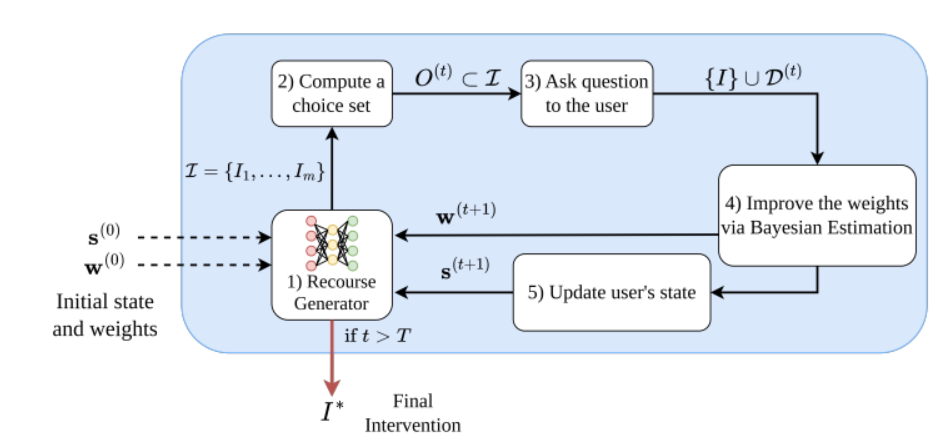
\includegraphics[width=0.75\linewidth]{images/detoni_et_al.png}
	\caption{Overview of PEAR - taken from Figure 1 in \textcite{detoniPersonalizedAlgorithmicRecourse2023}}
	\label{fig:detoni_et_al}
\end{figure}

They propose to compute a `choice set', a list of interventions for the user to responds with which intervention they would prefer. Bayesian estimation is then performed to update the weights, which correspond (a) user preferences over feature mutability and (b) the correlative effect of the value of $x_i$ on the cost of \textit{changing} $x_j$.\\

The methodology proposed in this thesis differs from \textcite{detoniPersonalizedAlgorithmicRecourse2023} in two key ways. Firstly, we adopt a fully causal setting (motivated and discussed in detail in chapter \ref{chapter:causal_recourse}). The cost function they use is shown below in Figure \ref{fig:detoni_et_al2}, where $a_i$ corresponds to the action (or change) on variable $i$ from $s_i$ to $s'_i$. The weights $w_i$ correspond to the user preferences over feature mutability and the the weights $w_{ij}$ correspond to the correlative effect of the value of $x_i$ on the cost of \textit{changing} $x_j$. However, as seen in Figure \ref{fig:detoni_et_al2}, the cost of an action of \textit{any} size on $x_i$ is affected by the current value of its parents multiplied by a weight. Regardless of the size of the change in variables $i$, its parents have a fixed effect. For example, in a scenario where income has a causal effect on savings, then having an income of £50,000 increases/reduces the cost of increasing savings by the same amount if we increase savings from £1 to £2 as it does if we increase savings from £1m to £2m. We do not believe that  this is a meaningful way to capture the effects of causal relations on the cost of changing feature values.

\begin{figure}[!htb]
	\centering
	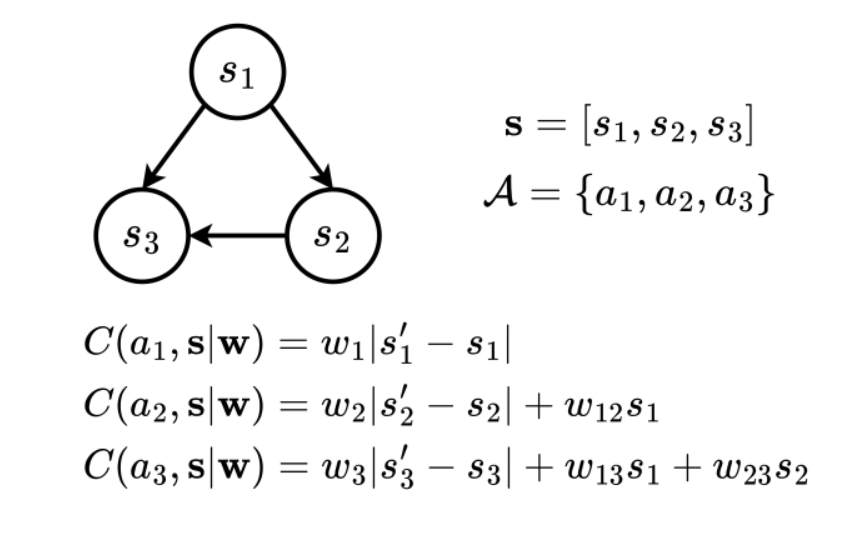
\includegraphics[width=0.5\linewidth]{images/detoni_et_al2.png}
	\caption{Cost function in PEAR - taken from Figure 2 in \textcite{detoniPersonalizedAlgorithmicRecourse2023}}
	\label{fig:detoni_et_al2}
\end{figure}

There are two major (and several minor) differences in the methodology presented in this thesis and \textcite{detoniPersonalizedAlgorithmicRecourse2023}. Firstly, as detailed in chapter \ref{chapter:causal_recourse}, we incorporate formal causal modelling \citep{pearl2016causal} in our cost function. Secondly, we learn an approximation of the structural causal model (SCM) that governs the world (and is the same for all individuals) as well as user preferences over feature mutability.


\section{Recourse methods}

There exist many different methods to generate recourse, which are reviewed in depth by \textcite{karimiSurveyAlgorithmicRecourse2022}. The methods used to generate recourse can broadly be grouped into three techniques.

\begin{itemize}
	\item \textit{Gradient-based optimisation}. When the cost function and constraint are both differentiable, gradient based approaches such as gradient descent (L-)BFGS and augmented Lagrangian methods (used in this thesis) are used to find alternative features $\mathbf{x}^*$.
	\item \textit{(Mixed) Integer Linear Programming}. In non-differentiable settings or where the features are discrete, tools such as (Mixed) Integer Linear Programming are used to solve for $\mathbf{x}^*$.
	\item \textit{Brute Force}. For cases with limited amounts of data and features and discrete data, brute force search through all possible values of $\mathbf{x}^*$ can be used \citep{vonkugelgenFairnessCausalAlgorithmic2022}.
\end{itemize}

This thesis aims to propose a methodology for learning cost functions, so to simplify the recourse problem we will only consider the case where continuous, actionable features are used. Examples of continuous, actionable features include income, a discrete, actionable feature would include level of education and a non-actionable feature would include age. As our data is continuous and actionable, we use gradient based optimisation (see section \ref{section:generating_recourse}) to generate recourse.